\documentclass[10pt,a4paper]{article}
\usepackage[utf8]{inputenc}
\usepackage[english]{babel}
\usepackage{amsmath}
\usepackage{amsfonts}
\usepackage{amssymb}
\usepackage{makeidx}
\usepackage{graphicx}
\usepackage[left=2cm,right=2cm,top=2cm,bottom=2cm]{geometry}
\author{George Biro}
\title{User Guide for Yet another Aurio analyseR}
\makeindex
\begin{document}
\maketitle
\tableofcontents
\pagebreak
\section{Introduction}
The yet another audio analyzer (yar) to do different measurements based on FFT using the sound layer. The software was tested by the E1DA ADC device (see https://e1dashz.wixsite.com/index/cosmos-adc), which has an 32 bits ADS and sampling up to 768kHz.
\section{Test Run}
To perform a simulated test with a 1kHz signal, with 100dB
\begin{verbatim}
./yar2.py --simfreq 1000 --simnoise 100 --plot sim --duration 10
\end{verbatim}
The software will run approx 10 seconds and will create a sim\_1000Hz.png file, what also will be displayed:
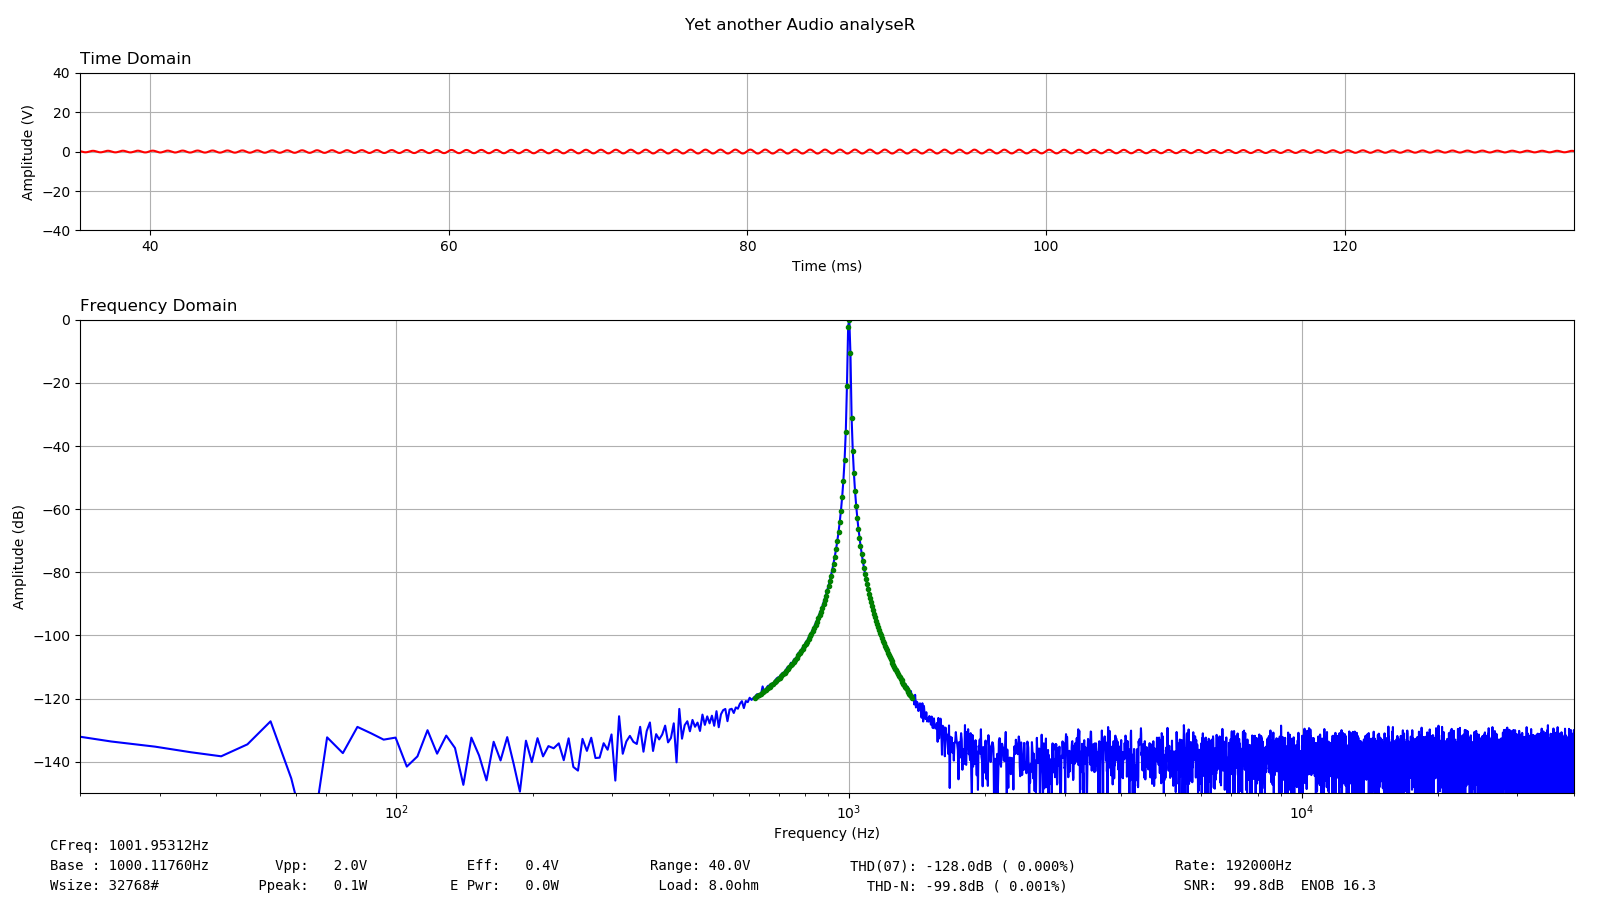
\includegraphics[width=\textwidth]{sim_1000Hz.png}
\section{Explanation of the measurements}
\subsection{CFreq}
Center frequency of the greatest FFT component
\subsection{Base}
Base or fundamental frequency computed by from the FFT.
\subsection{Wsize}
FFT window size
\subsection{Vpp}
Peak-to-peak voltage
\subsection{Ppeak}
Peak power
\subsection{Eff}
Effective or RMS voltage
\subsection{E-Pwr}
Effective power or RMS power
\subsection{Range}
Selected range
\subsection{Load}
Selected load (to compute power)
\subsection{THD(07)}
Computed THD value using 7 harmonics.
\subsection{THD-N}
Computed THD-N value
\subsection{Rate}
Sampling rate
\subsection{SNR}
Computde signal to noise ratio
\section{Command line switches}
\subsection{-h, --help}
To print help screen
\subsection{--list}
To print the list of audio devices. The program exits after all devices are listed
\subsection{--freq NUMBER}
The hardware sample rate, default is 192000Hz.
\subsection{--dev NUMBER}
Device to be used. The --list command displays the possible ids, default is 4. 
\subsection{--chsel NUMBER}
The selected channel (e.g. 0 for left side, 1 for right), default is 1.
\subsection{--chnum NUMBER}
The number of channels (e.g 1 for mono, 2 for stereo), default is 2.
\subsection{--chunk NUMBER}
The FFT window size, default is 32768. The system always takes the closest 2 power, so the 1000 will result 1024 automatically.
\subsection{--skip NUMBER}
Skip an amount of samples before doing FFT. Some audio devices has some bad behavior with the first some samples after opening it. Default is 1024.
\subsection{--adcrgn NUMBER}
The range of ADC chip, when is shows 0xff*. Default is 100V
\subsection{--adcres NUMBER}
The adc resolution, default is 32 (bits).
\subsection{--vrange NUMBER}
The voltage range in the time domain displaying in V, default is 40V.
\subsection{--frange NUMBER}
The frequency range in the frequency domain displaying in Hz, default is 40kHz. 
\subsection{--trange NUMBER}
The time range in the time domain displaying in ms, default is 100ms. The system automatically displays the mid.
\subsection{--wrange NUMBER}
The FFT range in the frequency domain displaying in dB, default is -150.
\subsection{--rload NUMBER} 
The size of the load resistor in ohm, to compute the power measurements from the voltage, default is 8ohm.
\subsection{--thd NUMBER}
Number of harmonics for THD calculation, default is 7. The THD(..) on the display changes accordingly to this settings.
\subsection{--duration NUMBER}
The software can be closed any time by the user, but after this time the system will exit. This is for help to run from scripts.
\subsection{--plot FILE}
The system automatically plots to file in case of stable fundamental frequency for 3sec (10sec in AVG mode). 

For example if the --plot TEST was invoked and the signal generator provides 1kHz signal after 3sec (10sec in AVG mode) a file will be written TEST\_1000Hz.png. If the signal generator changes to 400Hz and it is stable for 3sec (10sec in AVG mode) a new file will be written with the name TEST\_400Hz.png.
\subsection{--csv FILE}
The measurements are written into csv file. In case of stable fundamental frequency for 3sec (10sec in AVG mode). The program generates csv header if the file was not existing and appending the measurement to the generated or existing file.
\subsection{--window [bartlet|blackman|hamming|hanning|none]}
Select FFT window, default is hanning.
\subsection{--avg}
Doing FFT averaging. In case of change of fundamental frequency, the averaging starts from the beginning.
\subsection{--simfreq NUMBER}
For testing purposes only, feeding the software locally by fixed frequency.
\subsection{--simnoise NUMBER}
For testing purposes only, feeding the software locally by SNR dB. Use together with --simfreq options.
\subsection{--flttsh NUMBER}
Threshold in dB to determine filter for the spectral leakage at around the fundamental frequency. The system feeds an ideal sinus at fundamental frequency and the selected threshold determines a width or mask. This is displayed by the green dots on the frequency domain screen.
\subsection{--fnttsh NUMBER}
The fundamental voltage may computed by number of components, default is 3dB.
\subsection{--frqtsh NUMBER}
To compute the fundamental frequency, the selected in dB strongest components are used.
\subsection{--cftsh NUMBER}
For determine the spectral leakage, the system may use fundamental frequency or center frequency of the strongest FFT components.
\end{document}
